%%%%%%%%%%%%%%%%%%%%%%%%%%%%%%%%%%%%%%%%%
% Template latex pour les cours de physique sur femto-physique.fr
% J. ROUSSEL 
% 
%%%%%%%%%%%%%%%%%%%%%%%%%%%%%%%%%%%%%%%%%
%----------------------------------------------------------------------------------
%	PACKAGES AND OTHER DOCUMENT CONFIGURATIONS
%----------------------------------------------------------------------------------
\documentclass[
	a4paper, % Page size
	fontsize=10pt, % Base font size
	twoside=true, % Use different layouts for even and odd pages (in particular, if twoside=true, the margin column will be always on the outside)
	%open=any, % If twoside=true, uncomment this to force new chapters to start on any page, not only on right (odd) pages
	%chapterentrydots=true, % Uncomment to output dots from the chapter name to the page number in the table of contents
	numbers=noenddot, % Comment to output dots after chapter numbers; the most common values for this option are: enddot, noenddot and auto (see the KOMAScript documentation for an in-depth explanation)
]{kaobook}
% Choose the language
\ifxetexorluatex
	\usepackage{polyglossia}
	\setmainlanguage{french}
\else
	%\usepackage[english,french]{babel}
	\usepackage[french]{babel} % Load characters and hyphenation
\fi
\usepackage{csquotes}



% Load packages for testing
% \usepackage{blindtext}
% \usepackage{showframe} % Uncomment to show boxes around the text area, margin, header and footer
% \usepackage{showlabels} % Uncomment to output the content of \label commands to the document where they are used

% Load the bibliography package
\usepackage{kaobiblio}
\addbibresource{refOMP.bib}

% Load mathematical packages for theorems and related environments
\usepackage[framed=true]{kaotheorems}

% Load the package for hyperreferences
\usepackage{kaorefs}

% \makeindex[columns=3, title=Alphabetical Index, intoc] % Make LaTeX produce the files required to compile the index
% \makeglossaries % Make LaTeX produce the files required to compile the glossary
% \input{glossary.tex} % Include the glossary definitions
% \setlength{\nomitemsep}{-\parsep}.
\makenomenclature % Make LaTeX produce the files required to compile the nomenclature
%% This will add the subgroups
%----------------------------------------------
% \usepackage[separate-uncertainty=true,alsoload=synchem]{siunitx}
\usepackage[uncertainty-mode = separate]{siunitx}
\sisetup{locale = FR,group-digits = all} 
\DeclareSIUnit\mmHg{mmHg}
\DeclareSIUnit\bar{bar}
\DeclareSIUnit\torr{torr}
\DeclareSIUnit[quantity-product = {}] \degreeF{\text{\textdegree}F}

%----------------------------------------------
%% This will add the units
%----------------------------------------------
\newcommand{\nomunit}[1]{%
\renewcommand{\nomentryend}{\hspace*{\fill}#1}}
%----------------------------------------------

% Reset sidenote counter at chapters
% \counterwithin*{sidenote}{chapter}



% •••••••••••••••••••••••••••••••••••••••••••••••••••••••••••••••••••••••••••••••••••••
% 								| STYLES TIKZ |
% •••••••••••••••••••••••••••••••••••••••••••••••••••••••••••••••••••••••••••••••••••••
\tikzset{>=stealth,inner sep=1pt, outer sep=2pt}			
\tikzset{
	vecteur/.style={->,thick,color=black,smooth},
	systeme/.style={ellipse,inner sep=5pt,outer sep=5pt,fill=gray,draw,dashed,text={white}},
	echange/.style={color=cyan,thick,->,text={black}},
	gaz/.style={fill=SkyBlue!10,inner sep=1pt},
	liq/.style={top color=lightgray!50,bottom color=gray,text={white}},
	force/.style={->,>=latex,monBleu,nodes={monBleu},ultra thick,rounded corners=4pt,smooth,line cap=round},	
	source/.style={rectangle,minimum height=10mm,fill=blue!25,inner sep=5pt,text=blue},
	transfert/.style={decoration={markings,mark=at position 5mm with {\arrow[]{>}}},postaction=decorate},
	bloc/.style={rounded corners=4pt,color=white,ball color=lightgray,smooth},
	verre/.style={draw=SkyBlue,fill=SkyBlue!30},
	bob/.style={decoration={coil,aspect=0.5,segment length=2mm,amplitude=2mm}},	
	rayon/.style={draw=red!66,thick,line join=round}
	}	



%----------------------------------------------------------------------------------------
\begin{document}
\renewcommand{\labelitemi}{\tiny$\blacktriangleright$}
\renewcommand{\labelitemii}{\textbullet}

%----------------------------------------------------------------------------------------
%	BOOK INFORMATION
%----------------------------------------------------------------------------------------
\titlehead{
\begin{tikzpicture}[remember picture,overlay]
%%%%%%%%%%%%%%%%%%%% Background %%%%%%%%%%%%%%%%%%%%%%%%
\fill[monOrange] (current page.south west) rectangle (current page.north east);
%%%%%%%%%%%%%%%%%%%% Background Polygon %%%%%%%%%%%%%%%%%%%%
\foreach \i in {2.5,...,22}{
    \node[rounded corners,monOrange!60,draw,regular polygon,regular polygon sides=6, minimum size=\i cm,ultra thick] at ($(current page.west)+(2.5,-5)$) {} ;}
\foreach \i in {0.5,...,22}{
	\node[rounded corners,monOrange!60,draw,regular polygon,regular polygon sides=6, minimum size=\i cm,ultra thick] at ($(current page.north west)+(2.5,0)$) {} ;}
\foreach \i in {0.5,...,22}{
	\node[rounded corners,monOrange!90,draw,regular polygon,regular polygon sides=6, minimum size=\i cm,ultra thick] at ($(current page.north east)+(0,-9.5)$) {} ;}
\foreach \i in {21,...,6}{
	\node[monOrange!85,rounded corners,draw,regular polygon,regular polygon sides=6, minimum size=\i cm,ultra thick] at ($(current page.south east)+(-0.2,-0.45)$) {} ;}
%%%%%%%%%%%%%%%%%%%% Title of the Report %%%%%%%%%%%%%%%%%%%% 
\node[left,white,minimum width=0.625*\paperwidth,minimum height=3cm, rounded corners] at ($(current page.north east)+(0,-9.5)$){{\fontsize{25}{30} \selectfont \bfseries COURS DE PHYSIQUE}};
%%%%%%%%%%%%%%%%%%%% Subtitle %%%%%%%%%%%%%%%%%%%% 
\node[left,white,minimum width=0.625*\paperwidth,minimum height=2cm, rounded corners] at ($(current page.north east)+(0,-11)$){{\huge \textit{TEMPLATE LATEX}}};
%%%%%%%%%%%%%%%%%%%% Author Name %%%%%%%%%%%%%%%%%%%% 
\node[left,black!85,minimum width=0.625*\paperwidth,minimum height=2cm, rounded corners] at ($(current page.north east)+(0,-13)$){{\Large \textsc{Jimmy Roussel}}};
%%%%%%%%%%%%%%%%%%%% Year %%%%%%%%%%%%%%%%%%%% 
\node[rounded corners,text=monOrange,regular polygon,regular polygon sides=6, minimum size=2.5 cm,inner sep=0,ultra thick,fill=monOrange!60] at ($(current page.west)+(2.5,-5)$) {\LARGE \bfseries 2023};
\node[fill=white,ultra thick,draw=monOrange!60,text=monBleu,rounded corners,inner sep=4pt] at ($(current page.south)+(0,2)$) {\bfseries \href{https://femto-physique.fr/omp/}{femto-physique.fr/omp}} ;
\end{tikzpicture}
}
% \subject{}
\title[Cours sur les outils et méthodes scientifiques -- \href{https://femto-physique.fr}{femto-physique.fr}]{}

% \subtitle{}
\author[\textsc{Jimmy Roussel}, professeur agrégé à l'Ecole Nationale Supérieure de Chimie de Rennes]{}
\date{}

%----------------------------------------------------------------------------------------
% START of the pre-document content, uses roman numerals
% ---------------------------------------------------------------------------------------
\frontmatter 
%----------------------------------------------------------------------------------------
%	COPYRIGHT PAGE
%----------------------------------------------------------------------------------------
\makeatletter
\uppertitleback{\@plaintitle\\ \@plainauthor} % Header
\lowertitleback{
\textbf{Copyright} \copyright\ 2023 Jimmy Roussel\\
\ccbync\ Ce document est sous licence \emph{Creative Commons} «Attribution - Pas d’Utilisation Commerciale 4.0 International (CC BY-NC 4.0)».

Pour plus d'informations: \href{https://creativecommons.org/licenses/by-nc/4.0/}{creativecommons.org/licenses/by-nc/4.0/}
\medskip

Ce document est réalisé avec l'aide de \href{https://sourceforge.net/projects/koma-script/}{\KOMAScript} et  \href{ttps://www.latex-project.org/}{\LaTeX} en utilisant la classe \href{https://github.com/fmarotta/kaobook/}{kaobook}.
\medskip

\textbf{1\iere édition --} Janv. 2011

\textbf{Version en ligne --} \href{https://femto-physique.fr/omp/}{femto-physique.fr/omp}
}
\makeatother

%----------------------------------------------------------------------------------------
%	OUTPUT TITLE PAGE AND PREVIOUS
%----------------------------------------------------------------------------------------
% Note that \maketitle outputs the pages before here
\maketitle

%----------------------------------------------------------------------------------------
%	PREFACE
%----------------------------------------------------------------------------------------

\chapter*{Preface}
\addcontentsline{toc}{chapter}{Preface} % Add the preface to the table of contents as a chapter
Physics is a science that fundamentally relies on measurement and modeling. The physicist's toolkit must therefore include the tools and methods that enable them to:
\begin{enumerate}
    \item extract rational information from their measurements;
    \item approximate the behavior of a model system using mathematical analysis.
\end{enumerate}
This is why the course is divided into two parts: one focusing on measurement and another on mathematical concepts useful to physicists.

This course is aimed at a relatively broad audience, as it covers various tools used both in high school and higher education.


\begin{flushright}
	\textit{Jimmy Roussel}
\end{flushright}

\index{Préface}

%----------------------------------------------------------------------------------------
%	TABLE OF CONTENTS & LIST OF FIGURES/TABLES
%----------------------------------------------------------------------------------------

\begingroup % Local scope for the following commands

% Define the style for the TOC, LOF, and LOT
%\setstretch{1} % Uncomment to modify line spacing in the ToC
%\hypersetup{linkcolor=blue} % Uncomment to set the colour of links in the ToC
\setlength{\textheight}{230\hscale} % Manually adjust the height of the ToC pages

% Turn on compatibility mode for the etoc package
\etocstandarddisplaystyle % "toc display" as if etoc was not loaded
\etocstandardlines % "toc lines" as if etoc was not loaded

\tableofcontents % Output the table of contents

\listoffigures % Output the list of figures

% Comment both of the following lines to have the LOF and the LOT on different pages
\let\cleardoublepage\bigskip
\let\clearpage\bigskip

\listoftables % Output the list of tables

\endgroup
%----------------------------------------------------------------------------------------
%	MAIN BODY
%----------------------------------------------------------------------------------------
\mainmatter % Denotes the start of the main document content, resets page numbering and uses arabic numbers
\setchapterstyle{kao} % Choose the default chapter heading style

% -------- Outils d'analyse -------
\pagelayout{wide} % No margins
\addpart{Autour de la mesure}
\pagelayout{margin} % Restore margins

% !TEX encoding = UTF-8 Unicode 
\setchapterstyle{kao}
\setchapterpreamble[u]{\margintoc}
\chapter{UNITÉS ET DIMENSIONS}
\labch{unites_et_dimensions}


\blockquote[Bachelard]{Dis-moi comment l'on te cherche, je te dirai qui tu es}

\begin{center}
\textbf{Version en ligne}

\url{https://femto-physique.fr/omp/grandeurs-physiques.php}
\end{center}

\section[Dimension d'une grandeur]{Dimension d'une grandeurs physique}
\subsection{Grandeurs physiques}
Une grandeur physique est une quantité qui se rapporte à une propriété  et qui peut se mesurer. Or, \textbf{mesurer, c'est comparer}. C'est comparer à l'aide d'un instrument, une grandeur physique inconnue avec une grandeur de même nature -- on dira\textbf{ de même dimension} -- prise comme référence que l'on appelle \textbf{étalon}. 

Par exemple, le poids de Miss Univers peut être comparé à celui d'un étalon (1 kg par exemple) à l'aide d'une balance : le poids de Miss Univers est une grandeur physique. En revanche, sa beauté est une propriété subjective qui ne peut être mesurée compte tenu qu'il n'existe pas d'étalon de beauté. En d'autres termes, la beauté se rapporte à l'aspect physique mais ne relève pas de la Physique ; il ne s'agit pas d'une grandeur physique.

Lors du processus de mesure (mesurage) on effectue donc une comparaison entre un étalon (l'unité) et la grandeur à mesurer puis  l'on traduit le résultat par un chiffre (la mesure) assortie d'un intervalle définissant un certain niveau de confiance (l'incertitude) ainsi que l'unité\sidenote[][]{L'unité est indispensable ! Exprimer le résultat d'un calcul ou d'une mesure sans préciser l'unité n'a aucun sens.}
\[
X=x_\text{m}\pm\Delta x\quad\text{unité}
\] 
La détermination de la mesure et de l'incertitude fait l'objet d'un autre chapitre. Ici on s'intéresse au contenu dimensionnel des grandeurs physiques et du choix de l'unité.

\subsection{Notion de dimension}
En général, le résultat d'une mesure dépend de l'étalon utilisé. Par exemple, si l'on compare la longueur $\ell$ d'une règle de 1~m avec un décimètre, on obtient $\ell=10$~dm. Si l'on choisit un double décimètre comme étalon de mesure, on trouve $\ell=5$~ddm (double décimètre). La mesure est donc différente ($5\neq 10$) : on dit que  la longueur possède une dimension.
\newpage
\begin{kaobox}[frametitle=Dimension d'une grandeur]
Par définition, une grandeur physique $G$ a une dimension si sa mesure dépend du choix de l'étalon de mesure. Sa dimension est notée $[G]$.
\end{kaobox}
Il ne faut pas confondre cette notion avec l'unité qui est purement conventionnelle alors que la dimension est une propriété indépendante de tout système d'unités.

Deux grandeurs ont même dimension si on peut les comparer. C'est pourquoi le rayon d'un cercle et son périmètre ont même dimension, car je peux en faire la mesure avec le même étalon (par exemple un fil souple d'une certaine longueur). Ici il s'agit de la dimension [longueur].

Il existe également des grandeurs physiques sans dimension (on dit aussi adimensionnées). Dans ce cas la dimension est noté $[G]=1$. Par exemple, l'angle $\theta$ d'un secteur AOB est une grandeur que l'on peut mesurer comme suit : traçons un cercle de centre O et de rayon  $r$. Les droites (OA) et (OB) coupent le cercle en deux points A' et B'. L'angle se mesure en faisant le rapport de la longueur d'arc $\arcdecercle{A'B'}$ et du rayon du cercle.
\begin{marginfigure}
\centering
	\begin{tikzpicture}
	\draw (10:3)node{•}node[right=5pt]{B}--(0,0)node{•}node[left=5pt]{O}--(-10:2)node{•}node[right=5pt]{A};
	\draw[dashed] (0,0) circle(1);
	\draw[thick,blue] (-10:1)node[below,fill=white]{\small A'} arc(-10:10:1)node[above,fill=white]{\small B'};
	\draw (0,0)--(90:1)node[midway,fill=white]{$r$};
	\draw (0:1)node[right=5pt]{$\theta$};
	\end{tikzpicture}
\caption{Définition de l'angle plan.}
\labfig{définition_de_l_angle_plan}
\end{marginfigure}
\[
	\theta\stackrel{\text{def}}= \dfrac{\arcdecercle{A'B'}}{r}
\]
\begin{margintable}
\centering
\footnotesize
\caption{Symbole donné aux dimensions des grandeurs de base.}
\labtab{lettre_donnee_aux_dimensions_des_grandeurs_de_base}
	\begin{tabular}{lc}
		\toprule
		\textbf{Dimension}		& \textbf{Symbole}	\\
		Longueur				& L			\\
		Masse					& M			\\
		Temps					& T			\\
		Intensité électrique	& I			\\
		Température				& $\Theta$	\\	
		Quantité de matière		& N\\
		\bottomrule
	\end{tabular}
\end{margintable}
On constate donc que si l'on double le rayon du cercle, la longueur d'arc double également de sorte que l'angle ne dépend pas de la taille du cercle. Il est alors assez évident que si l'on décide de mesurer les distances en centimètre, en pouce, ou dans n'importe quel système d'unités, le résultat de l'angle $\theta$ ne changera pas. \textbf{L'angle est donc sans dimension}. De la même manière, une grandeur définie comme le rapport de deux grandeurs de même dimension, ne présente pas de dimension. 

Enfin, par commodité, on a donné un nom spécifique à  certaines dimensions (cf. \reftab{lettre_donnee_aux_dimensions_des_grandeurs_de_base}).



\subsection{Équation aux dimensions}	
Une loi physique affirme l'égalité de deux grandeurs qui sont nécessairement de même nature. Une loi physique est donc aussi une relation entre différentes dimensions : on parle d'\textbf{équation aux dimensions}. 
Voyons comment obtenir ces équations aux dimensions sur quelques exemples. 
\begin{description}
	\item[La vitesse :] d'après la définition $v_x\stackrel{\text{def}}=\mathrm{d}x/\mathrm{d}t$, on déduit 
	\[[v]=\mathrm{LT^{-1}}\]
	\item[L'accélération :] la définition $a_x\stackrel{\text{def}}=\mathrm{d}v_x/\mathrm{d}t$ donne 
	\[[a]=\frac{[v]}{\text{T}}=\mathrm{LT^{-2}}\]
	\item[La force :] en vertu de la deuxième loi de Newton $F=ma$ on a 
	\[[\text{F}]=\mathrm{MLT^{-2}}\] 
	\item[La constante des gaz parfaits :] on peut obtenir sa dimension à partir de la loi du gaz parfait $pV=nRT$.  
	\[ [R]=\frac{[p][V]}{[n][T]}=\frac{[F]}{\mathrm{L^{2}}}\times\frac{\mathrm{L^3}}{N\Theta}=
	\mathrm{ML^2}\mathrm{T^{-2}}\Theta^{-1}\mathrm{N^{-1}}\]	
	\item[Le champ magnétique :] par définition du champ magnétique, une particule de charge électrique 
	$q$ se déplaçant à la vitesse $\overrightarrow{v}$ dans un champ magnétique $\overrightarrow{B}$ subit une force 
	$\overrightarrow{F}=q\overrightarrow{v}\wedge\overrightarrow{B}$, d'où
	\[ [B]=\frac{[F]}{[q][v]}=\frac{\mathrm{MLT}^{-2}}{\mathrm{IT}\times \mathrm{LT}^{-1}}=\mathrm{MT}^{-2}\mathrm{I}^{-1}\]
\end{description}



\section[Le SI]{Le Système international d'unités}
Comme on l'a déjà dit, mesurer c'est comparer une grandeur physique avec un étalon qui définit l'\textbf{unité de mesure}. Celle-ci relevant d'un choix arbitraire il faut bien  \textbf{convenir} d'un système d'unités pour pouvoir communiquer (transactions commerciales, rapports scientifiques, etc.). La bonne idée consiste alors à choisir des étalons dont la définition est indépendante du lieu et du temps et avec lesquels on peut construire toutes les unités. C'est l'ambition du Système international d'unités (SI) adopté par quasiment tous les pays\sidenote{Trois pays n'ont pas encore adopté officiellement le système métrique : le Libéria, la Birmanie et… les Etats-Unis.}. Né officiellement en 1960, il s'agit d'une extension de l'ancien système MKSA. 

 
\subsection{Les unités de base} 
\begin{marginfigure}[*6]
\centering
	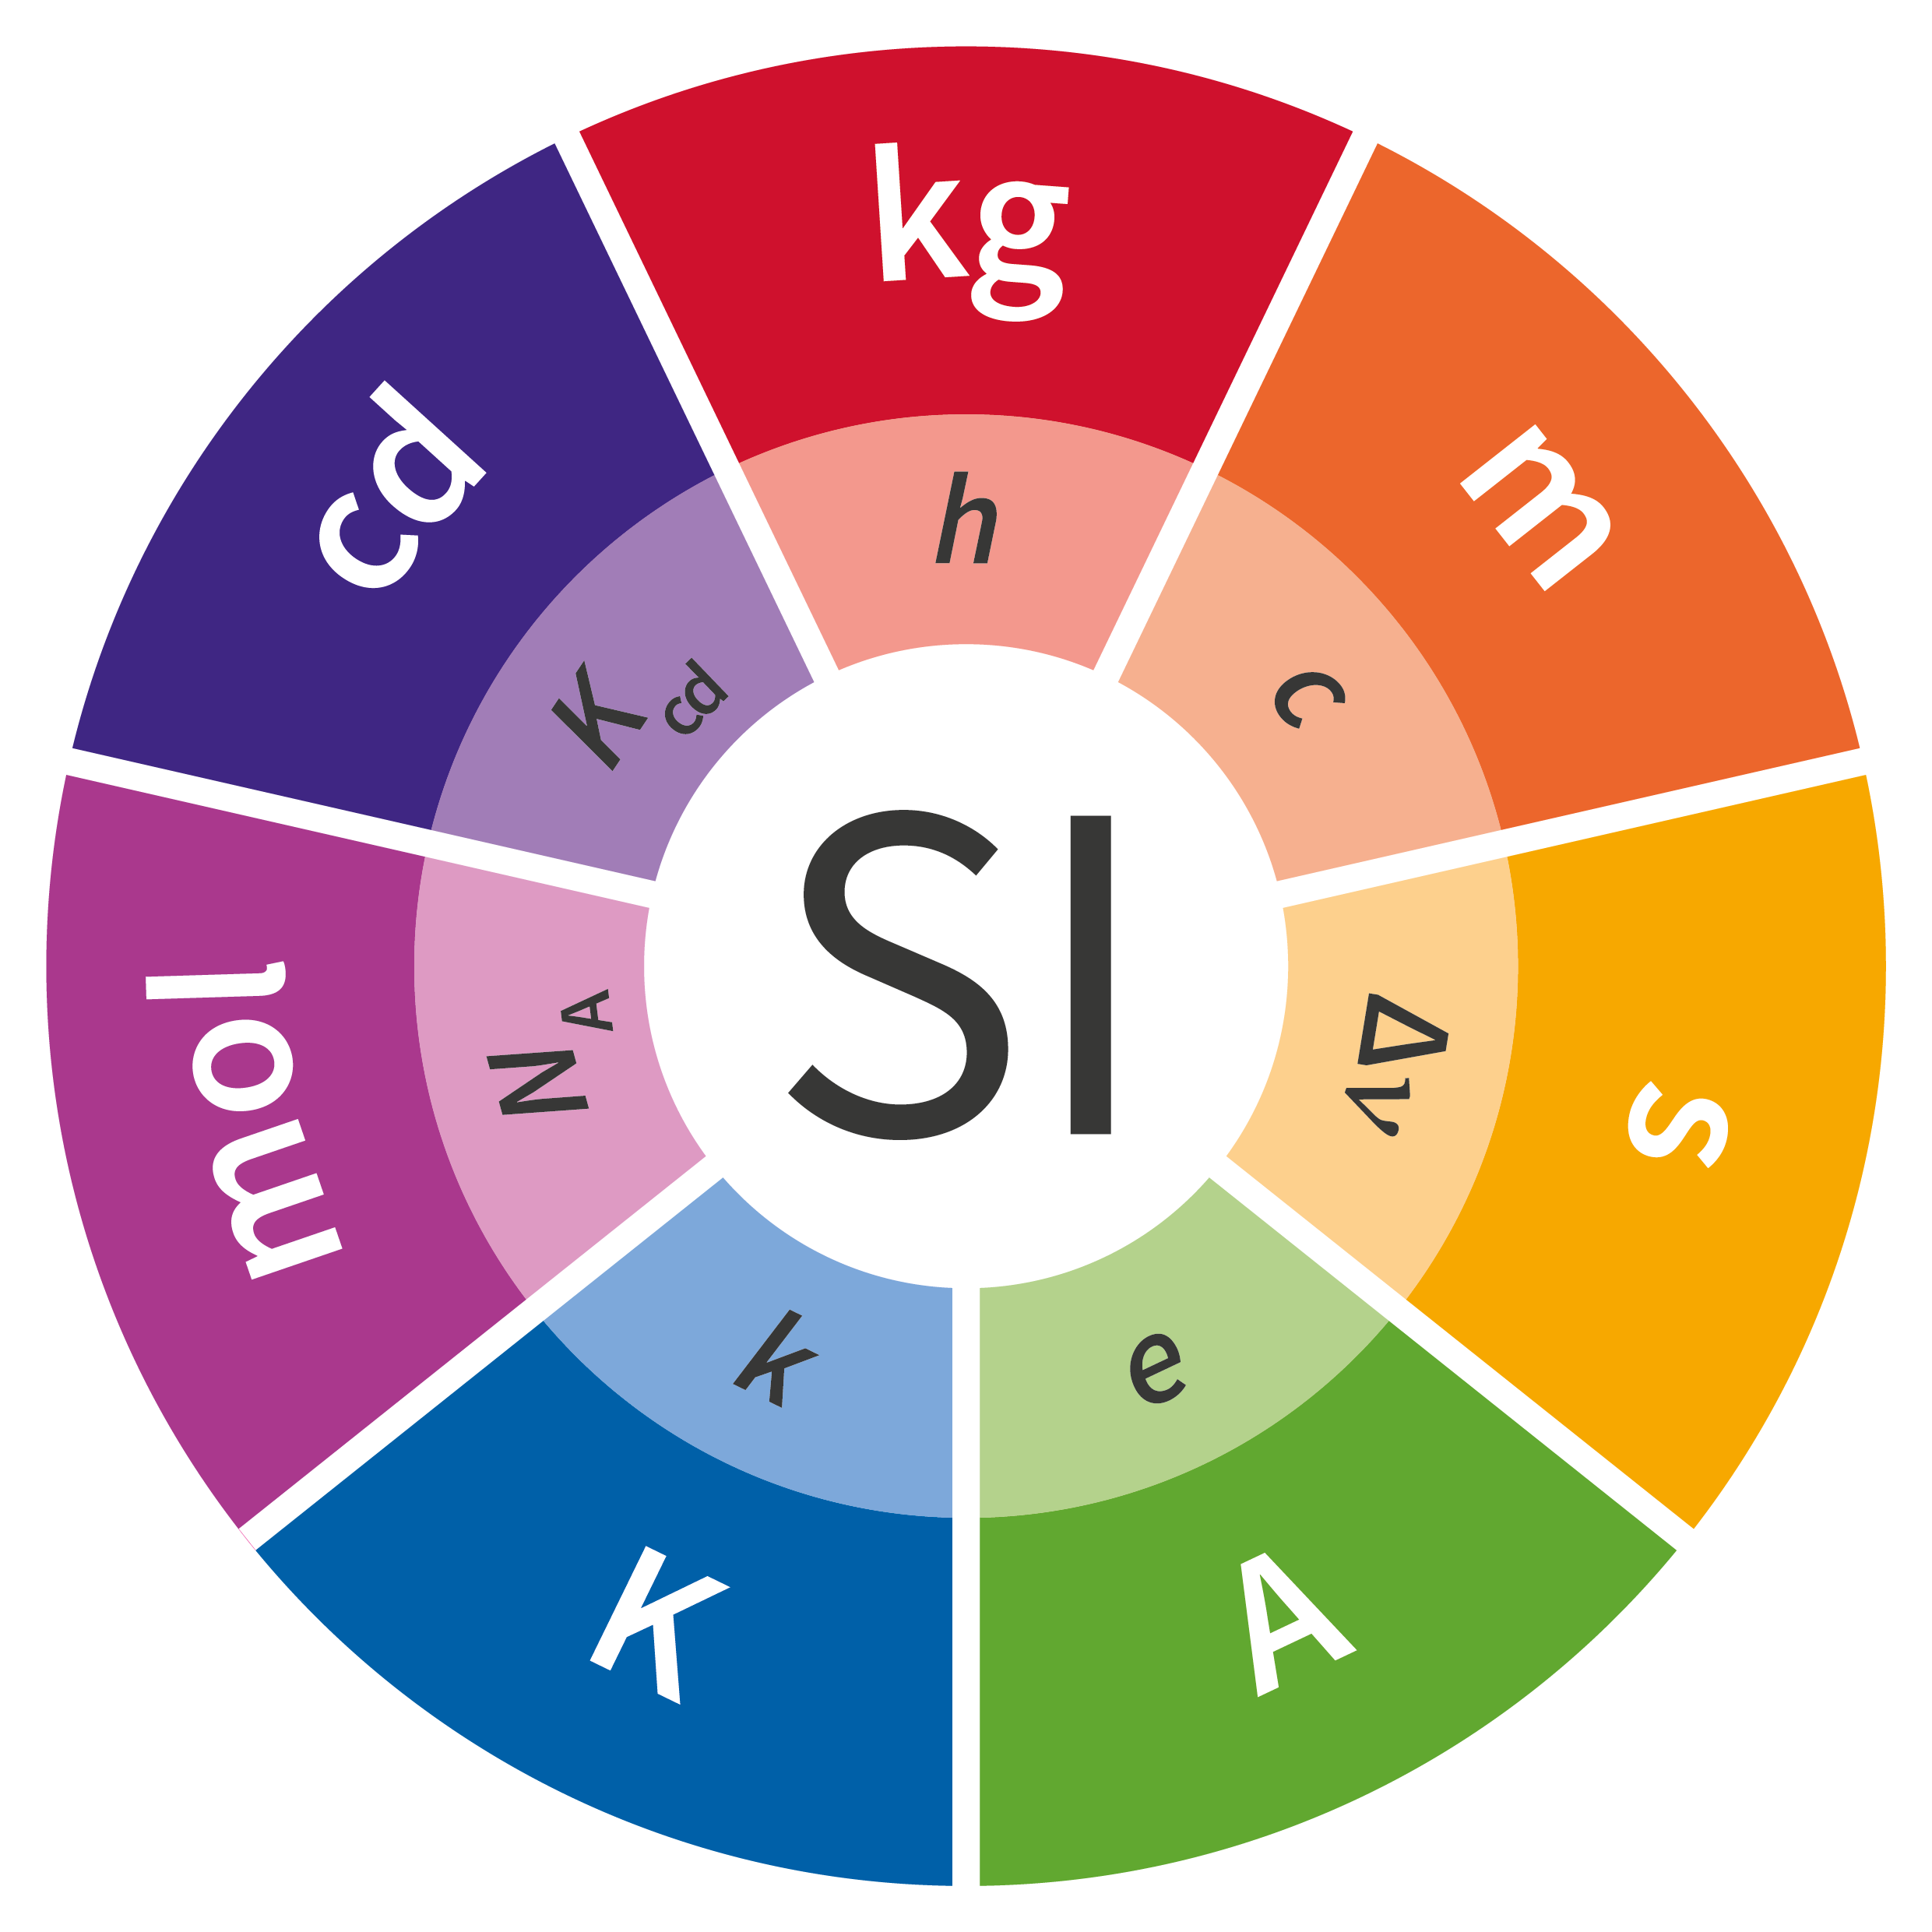
\includegraphics[width=5cm]{img/SI-Illustration-Constants-Colour-Full.png}
\caption{Le SI et ses 7 unités fondamentales liées aux 7 constantes universelles.}
\labfig{title_name}
\end{marginfigure}
Le (SI) forme un système cohérent reposant sur \textbf{sept unités de base} (\emph{cf.} \reftab{sept_unites_de_base}) indépendants du point de vue dimensionnel. 
\begin{table}[ht!]
	\centering
	\footnotesize
	\caption{Les sept unités de base du Système internationale d'unités.}
	\labtab{sept_unites_de_base}	
	\begin{tabular}{lcrr}
		\toprule
		\textbf{Dimension}		& \textbf{Symbole}	& \textbf{Unité SI}	&\textbf{Symbole}\\
		Longueur							& L									& mètre						& m\\
		Masse									& M									& kilogramme			& kg\\
		Temps									& T									& seconde					& s\\
		Intensité électrique	& I									& ampère					& A\\
		Température						& $\Theta$					& kelvin					& K\\
		Quantité de matière		& N									& mole						& mol\\
		Intensité lumineuse		& J									& candela					&cd\\
		\bottomrule
		\end{tabular}
\end{table}
Depuis le 20 mai 2019, les unités du SI sont définies à partir de sept constantes de la nature auxquelles on donne une valeur fixe. Les sept constantes sur lesquelles repose le Système international d'unités sont
\begin{itemize}
\item la fréquence de la transition hyperfine du césium 133 \(\Delta \nu_\textsf{Cs}=9\,192\,631\,770\,\mathrm{Hz}\) qui permet de définir la seconde ;
\item la vitesse de la lumière dans le vide \(c=299~792~458\,\mathrm{m.s^{-1}}\) qui permet de relier le mètre à la seconde ;
\item la constante de Planck \(h=6{,}626~070~15\cdot 10^{-34}\,\mathrm{kg.m^2.s^{-1}}\) qui définit indirectement le kilogramme ;
\item la charge élémentaire \(e=1{,}602~176~634\cdot 10^{-19}\,\mathrm{C}\) qui fixe l'ampère puisque \(1\,\mathrm{C}=1\,\mathrm{A.s}\) ;
\item la constante de Boltzmann \(k_\text{B}=1{,}380~649 \cdot 10^{-23} \, \mathrm{J.K^{-1} } \) qui relie le kelvin aux unités mécaniques ;
\item la constante d'Avogadro \(N_\text{A}=6{,}022~140~76\cdot 10^{23}\,\mathrm{mol^{-1}}\) qui donne le nombre exact d'entités élémentaires (atomes, molécules, ions, etc.) formant une mole ;
\item Enfin, l'efficacité lumineuse \(K_{cd}=683\,\mathrm{lumen.W^{-1}}\) pour un rayonnement monochromatique de longueur d'onde\sidenote[][]{Cette longueur d'onde correspond au maximum de sensibilité de l'œil humain.} \(\lambda=555\,\mathrm{nm}\). Cette constante relie les grandeurs sensorielles (intensité en candela, éclairement en lux, flux lumineux en lumen) aux grandeurs énergétiques de la lumière (intensité en watt par stéradian, éclairement en watt par mètre carré, flux en watt).
\end{itemize}
Notez que ces constantes sont des grandeurs physiques sans incertitude. En revanche, certaines grandeurs auparavant fixées (avant mai 2019) retrouvent leur statut de grandeur expérimentale. Par exemple, une mole de carbone 12 pesait auparavant 12~g par définition ; dorénavant sa valeur n'est plus connue exactement. Elle présente donc une incertitude.



%\begin{description}
%	\item[Le mètre] est relié à la seconde \emph{via} l'invariance de la vitesse de la lumière dans le vide. Par définition, la distance parcourue par la lumière dans le vide pendant une seconde vaut $L=299\,792\,458\, \rm m$
%
%\remarque{le mètre a connu en deux siècles quatre définitions successives. Initialement, le mètre était défini à partir de la longueur du méridien terrestre supposé invariable: $L=40\,000\;{\rm km}$. Aujourd'hui, avec l'étalon mètre actuel (lié à l'étalon seconde) $L=40\,008,08\;{\rm km}$ ; la différence est donc imperceptible pour un utilisateur courant.}
%	
%	\item[Le kilogramme] est la masse d'un bloc cylindrique de Platine irridié (90\%Pt-10\%Ir) conservé au pavillon de Breteuil (Sèvres) depuis 1889. 
%	
%	\remarque{cet étalon se dégrade par usure et contamination ; c'est pourquoi il est envisagé de changer de définition du kg et de définir cette unité à partir de la constante de Planck $h$.}
%
%	\item[La seconde] est la durée de $9\,192\,631\,770$ périodes de la radiation correspondante à la transition entre les deux niveaux hyperfins de l'état fondamental de l'atome $\mathrm{_{133}Cs}$ au repos dans le référentiel d'étude.
%	
%	\remarque{initialement la seconde était définie à partir du jour solaire moyen J par la relation $J=86400\,{\rm s}$. Aujourd'hui, avec la définition de l'étalon seconde, on a $J=86400,003\,{\rm s}$.}
%
%	\item[L'ampère] est défini à partir de la force magnétique de Laplace et permet d'établir à $10^{-7}$ près les principaux étalons du domaine électrique. Un ampère est l'intensité du courant qui fait apparaître une force de $2.10^{-7}\;\mathrm{N}$ entre deux conducteurs filiformes rectilignes infinis distants de $1\;\mathrm{m}$, parcourus par ce courant électrique.
%	
%	\remarque{cette définition fixe les valeurs de la perméabilité magnétique et de la permittivité du vide à
%			\[\mu_{0}=4\pi.10^{-7}\;\mathrm{H.m^{-1}}\quad\text{et}\quad\epsilon_0=\frac{1}{\mu_0 c^2}\]
%	Notez qu'il est prévu de redéfinir l'ampère à partir de la charge de l'électron $e$ ce qui aura pour effet de fixer la valeur de $e$ mais de rendre à $\mu_0$ et à $\epsilon_0$ leur statut de constantes expérimentales.}
%	
%	\item[Le kelvin] se rapporte à la loi du gaz parfait. Par définition du kelvin, la température d'un gaz parfait en équilibre avec l'eau dans ses trois états (le point triple de l'eau) vaut $273,16\;\mathrm{K}$.
%	
%	\remarque{la future définition du kelvin fixera la valeur de la constante de Boltzmann $k_{\rm B}$.}
%	
%	\item[La mole] est la quantité d'atomes contenue dans 12~g de carbone 12. 
%	
%	\remarque{l'imprécision de cet étalon est donc liée à celle de la masse. Pour pallier cet inconvénient, il est envisagé de définir la mole en fixant la valeur du nombre d'Avogadro.}
%
%	\item[La candela] est l'unité donnant l'intensité lumineuse d'une source dans une direction donnée. Par définition, 1~cd est intensité lumineuse d'une lumière verte de fréquence $\nu=540.10^{12}\;\mathrm{Hz}$ rayonnant $\dfrac{1}{683}\;\mathrm{W.sr^{-1}}$.
%\end{description}


\subsection{Les unités dérivées}
Les sept unités de base du système international sont les «unités fondamentales» à partir desquelles sont obtenues par combinaison toutes les autres unités, dites \textbf{unités dérivées}. Certaines d'entre-elles se sont vues attribuer un nom qui rappelle une personnalité scientifique: newton, pascal, joule, volt, tesla, henry etc.
\begin{table}[htbp]
	\caption{Quelques unités dérivées.}
	\labtab{unites-derivees}
	\footnotesize
	\begin{tabular}{lrlr}
	\toprule
	\textbf{Grandeur}					&\textbf{Unité SI}
	&
	\textbf{Grandeur}					&\textbf{Unité SI} \\
	\midrule
	aire								& $\mathrm{m^{2}}$ 
	&énergies 							& J	(joule)\\	

	volume								& $\mathrm{m^{3}}$  
	&pression							& Pa (pascal)\\

	masse molaire						& $\mathrm{kg.mol^{-1}}$ 
	&tension								& V (volt)\\

	masse volumique 					& $\mathrm{kg.m^{-3}}$ 
	&charge électrique					& C (coulomb)\\

	fréquence							& Hz (hertz)
	&résistance électrique				& $\Omega$ (ohm)\\

	vitesse (scalaire)					& $\mathrm{m.s^{-1}}$ 
	&champ électrique					& $\mathrm{V.m^{-1}}$\\

	vitesse angulaire, pulsation		& $\mathrm{rad.s^{-1}}$ 
	&conductance électrique				& S (siemens)\\

	accélération (scalaire) 			& $\mathrm{m.s^{-2}}$ 
	&capacité électrique					& F (farad)\\

	force d'interaction 				& N (newton)
	&inductance							& H (henry)\\

	puissance mécanique					& W (watt)	
	&champ magnétique					& T (tesla)\\	   
	\bottomrule
	\end{tabular}
\end{table}
Il peut donc y avoir différentes façons d'exprimer la même unité.	

\begin{kaoexample}[frametitle=Exemple : unités de la pression]
La pression s'exprime en pascal (Pa) dans le système international. Etant donné que la pression représente une force par unité de surface on peut aussi l'exprimer en $\mathrm{N/m^2}$. Par ailleurs, on sait d'après l'équation aux dimensions $\mathrm{F=MLT^{-2}}$, que $1\;\mathrm{N}=1\;\mathrm{kg.m.s^{-2}}$ d'où l'on déduit 
\[
1\;\mathrm{Pa}=1\;\mathrm{N.m^{-2}}=1\;\mathrm{kg.m^{-1}.s^{-2}}
\]
\end{kaoexample} 
 
\begin{kaoremark}
Il existe une dernière classe d'unités qu'on appelle unités supplémentaires. Cette classe contient deux unités sans dimension : le radian (rad), unité de l'angle plan, et le stéradian (sr), unité d'angle solide.
\end{kaoremark} 


\subsection{Préfixes SI}	
Enfin, on utilise parfois des préfixes multiplicateurs pour remplacer les puissances de 10 : 
\begin{table}[h!tbp]
	\caption{Préfixes multiplicateurs.}
	\labtab{prefixe-multiplicateurs}
	\footnotesize
\begin{tabular}{lcccccccc}
\toprule
Valeur &	$10^{-18}$ &	$10^{-15}$ &	$10^{-12}$ &	$10^{-9}$ &	$10^{-6}$ &	$10^{-3}$ &	$10^{-2}$ &	$10^{-1}$ \\
Préfixe &	atto &	femto &	pico &	nano &	micro &	milli &centi & déci \\
Symbole	& a	& f	& p	& n	& $\mu$	& m & c & d	\\
\midrule
\midrule
Valeur &	$10$	& $10^{2}$	& $10^{3}$	& $10^{6}$	& $10^{9}$	& $10^{12}$	& $10^{15}$	& $10^{18}$ \\
Préfixe &	déca	& hecto		& kilo 		& Mega		& Giga 		& Tera 		& Peta 		&	Exa \\
Symbole	& da& h	& k	& M	& G	& T	& P &	E \\
\bottomrule
\end{tabular}
\end{table}

\section{Analyse dimensionnelle}
Analyser le contenu dimensionnel d'une relation permet de rendre bien des services. En voici un petit tour d'horizon ...
\subsection{Vérifier une formule}
Une loi physique impose une contrainte qui n'existe pas en mathématique ; elle doit être \textbf{homogène}, c'est-à-dire constituée de termes de même dimension. Sommer deux grandeurs de dimension différente n'a aucun sens en physique. Ainsi pour vérifier une loi physique, la première chose à faire est de vérifier l'homogénéité !	
\begin{kaobox}[frametitle=Vérifier une formule]
	Toute formule non homogène est nécessairement fausse. On retiendra quelques règles :
\begin{itemize}
	\item dans $\sin x$, $\cos x$, $\mathrm{e}^x$, $\ln x$ et $\log x$ la grandeur $x$ doit être sans dimension ;
	\item dans $1+x$, la grandeur $x$ doit être sans dimension ;
	\item dans $1+x/y$, les grandeurs $x$ et $y$ sont de même dimension.
\end{itemize}
\end{kaobox}


\exercice{La période d'oscillation d'un pendule simple dépend de sa longueur $\ell$, du champ de pesanteur $g$ et de l'amplitude angulaire $\theta_\text{max}$ des oscillations. On propose plusieurs formules ; préciser celles qui ne sont pas homogènes :
\begin{multicols}{2}
	\begin{itemize}[label=$\square$]
		\item $T=2\pi\sqrt{\dfrac{\ell+\theta_\text{max}}{g-\theta_\text{max}}}$
		\item $T=2\pi\sqrt{\dfrac{\ell}{g\theta_\text{max}}}$
		\item $T=2\pi\sqrt{\dfrac{\ell}{g}}\left(1+\dfrac{{\theta_\text{max}}^2}{16}\right)$
		\item $T=2\pi\sqrt{\dfrac{\ell}{g}}\left(1+\dfrac{\theta_\text{max}}{\ell}\right)$
	\end{itemize}
\end{multicols}}

Bien entendu, cela ne signifie pas qu'une formule homogène soit forcément exacte, mais cela permet déjà de trier ce qui n'a aucun sens physique de ce qui peut en avoir. De manière générale, l'analyse dimensionnelle est un outil de réfutation, pas de validation.

\begin{kaoremark}
Il faut prendre garde à certaines formules qui mélangent expressions numériques et littérales. Par exemple, le pH d'une solution acido-basique diluée est souvent défini par 
	\[\text{pH}=-\log\left[\mathsf{H_3O^+}\right]\]
Or la concentration n'est pas sans dimension ce qui suggère que cette formule est non-homogène. En réalité cette formule n'obéit pas à la règle élémentaire qui veut que toute relation soit indépendante du système d'unités. En effet, dans la formule qui donne le pH, il est sous entendu qu'il faut exprimer $\left[\mathsf{H_3O^+}\right]$ en mol.L$^{-1}$. Si l'on veut donner la relation qui donne le pH quel que soit le système d'unités on écrira plutôt
	\[\text{pH}=-\log\frac{\left[\mathsf{H_3O^+}\right]}{c^{\circ}}\]
où $c^{\circ}$ désigne la concentration standard. Dans le SI, $c^{\circ}=1000\;\mathrm{mol.m^{-3}}$ mais si l'on décide d'exprimer les concentrations en mol.L$^{-1}$, on a $c^{\circ}=1\;\mathrm{mol.L^{-1}}$ et dans ce cas la tentation est grande de faire disparaître cette constante par commodité. Mais cela ne doit pas nous faire oublier sa présence.
\end{kaoremark} 



\subsection{Conversion d'unités}
L'équation aux dimensions étant indépendante du système d'unités, elle est très utile quand il faut convertir une unité d'un système vers celle d'un autre système. 

\begin{kaoexample}[frametitle=Exemple : la dyne]
Dans le Système International, la force s'exprime en newton alors qu'elle s'exprime en dyne dans le Système CGS (cm, gramme, seconde). Combien de newton vaut 1 dyne ?

L'équation aux dimensions $[\text{Force}]=\mathrm{MLT^{-2}}$ doit être vérifiée dans tout système d'unités. On a donc
	\[\text{1 newton}=\mathrm{1\, kg.m.s^{-2}}\quad\text{et}\quad \text{1 dyne}=\mathrm{1\, g.cm.s^{-2}}\]
Ainsi on en déduit la conversion : 
	\[1\;\mathrm{newton}=10^5\;\mathrm{dynes}\]
\end{kaoexample} 

\subsection{Modéliser}
L'analyse dimensionnelle permet de prévoir la forme d'une loi si l'on sait quels sont les paramètres pertinents du problème.

Supposons par exemple que nous cherchions à exprimer une grandeur $G$ en fonction de 2 paramètres pertinents indépendants $p_{1}$ et $p_{2}$. La méthode consiste alors à trouver comment multiplier $p_1$ et $p_2$ pour former une grandeur de  même dimension que $G$. On écrit donc 
	\[G=\mathrm{C^{te}}{p_1}^\alpha\,{p_2}^\beta\]
où $\alpha$ et $\beta$ sont des facteurs que l'on détermine grâce à l'équation aux dimensions. Une fois ces constantes déterminées, on peut proposer la forme générale de la loi recherchée.

\begin{kaoexample}[frametitle=Exemple : période d'oscillation $T$ d'un pendule simple]
On suppose que la période $T$ dépend de la masse $m$, du champ de pesanteur $g$ et de la longueur $\ell$ du pendule : $T=f(m,g,\ell)$. On écrit alors 
	\[T=\mathrm{C^{te}}m^{\alpha}\,g^{\beta}\,\ell^{\gamma}\]	
où $\mathrm{C^{te}}$ est un facteur adimensioné. Cela nous donne l'équation aux dimensions 
	\[\mathrm{T}=\mathrm{M}^{\alpha}\mathrm{L}^{\gamma+\beta}\mathrm{T}^{-2\beta}\]
La loi devant être homogène on doit poser $\alpha=0$, $\beta=-1/2$ et $\gamma=1/2$. La forme générale est donc 
	\[T=\mathrm{C^{te}}\sqrt{\frac{\ell}{g}}\]
Attention, ce n'est pas parce que l'on trouve une loi qu'elle est juste ! L'analyse dimensionnelle nous dit simplement que la loi est correcte en termes de dimension. C'est à l'expérience de confirmer ou d'infirmer l'analyse. Par exemple, dans le cas du pendule, supposer comme nous l'avons fait, que la période du pendule ne dépend pas de l'amplitude des oscillations est en contradiction avec les faits\footnote{On peut montrer que cette propriété n'est correcte que si les angles sont petits.}. Il faut alors introduire l'amplitude $\theta_0$ des oscillations dans l'analyse dimensionnelle : 
	\[T=f(m,g,\ell,\theta_0)
	\quad\Longrightarrow\quad
	T=\mathrm{C^{te}}m^{\alpha}\,g^{\beta}\,\ell^{\gamma}{\theta_0}^\delta\]	
d'où l'équation aux dimensions 
	\[\mathrm{T}=\mathrm{M}^{\alpha}\mathrm{L}^{\gamma+\beta}\mathrm{T}^{-2\beta}\]
identique à la précédente. On trouve donc les mêmes résultats ($\alpha=0$, $\beta=-1/2$ et $\gamma=1/2$) et $\delta$ peut prendre des valeurs quelconque. En d'autres termes on peut écrire la période ainsi
\[
	T=\sqrt{\frac{\ell}{g}}(a_0+a_1\,\theta_0+a_2\,{\theta_0}^2+\ldots+a_p\,{\theta_0}^p+\ldots)
\]
où les exposants peuvent être quelconques de sorte que la forme la plus générale est 
\[T=\sqrt{\frac{\ell}{g}}f(\theta_0)\]
\end{kaoexample} 
	
Notez que l'analyse dimensionnelle ne permet pas de déterminer complètement la loi recherchée. Dans le meilleur des cas, une constante adimensionnée est à déterminer de façon empirique.




% !TEX encoding = UTF-8
\setchapterstyle{kao}
\setchapterpreamble[u]{\margintoc}
\chapter{MESURES ET INCERTITUDES}
\labch{mesures_et_incertitudes}


\blockquote[Edgar Morin]{La connaissance progresse en intégrant en elle l'incertitude, non en l'exorcisant}

Accéder à une valeur objective de la réalité sans erreur est tout simplement impossible. L'erreur fait parti de l'opération de mesure. Une des forces de la science est d'avoir mis au point des outils qui permettent d'\textbf{estimer} cette erreur.

\begin{center}
\textbf{Version en ligne}

\url{https://femto-physique.fr/omp/mesures-et-incertitudes.php}
\end{center}





\section{Mesurer c'est évaluer}%(fold)

\subsection{Notion d'erreur et d'incertitude}[Erreur et incertitude]%(fold)
\begin{kaoexample}[frametitle=Expérience]
Mesurons, à l'aide d'un chronomètre, la durée $t$ correspondant à 2,5 périodes d'oscillation d'un pendule simple (5 passages à la verticale). En faisant faire cette même mesure par différents élèves on trouve 
\begin{center}
\begin{tabular}{c|cccc}
mesure \no&1&2&3&4\\
\hline
durée $t$&3,62~s&3,47~s&3,44~s&3,30~s\\
\end{tabular}	
\end{center}
\end{kaoexample} 
L'expérience précédente montre que les résultats sont différents ce qui traduit l'existence \textbf{d'erreurs de mesure}.  L'erreur faite lors de la mesure d'une grandeur $x$ est l'écart entre la valeur mesurée ($x_i$) et sa valeur vraie ($x_\text{vraie}$), laquelle est unique mais inaccessible. Elle présente deux composantes.
\begin{description}
	\item[Erreur aléatoire] L'erreur aléatoire $\epsilon_a$ provient des variations temporelles et spatiales \textbf{non prévisibles} de grandeurs d'influence\sidenote{Par exemple, le soin avec lequel sont effectuées les mesures, la température de la pièce, la fidélité de l'appareil de mesure, etc.}. Elle est définie par  
	\[\epsilon_a=x_i-\overline{x}\]
	où $\overline{x}$ est la moyenne des mesures obtenue en répétant $N$ fois la même expérience avec $N\to \infty$.
	\item[Erreur systématique] L'erreur systématique\sidenote{On dit aussi \emph{biais}.} $\epsilon_s$ est un \textbf{décalage constant} dont l'origine peut être d'ordre théorique ou expérimentale\sidenote{Exemple de biais: influence du mode opératoire, problème de calibrage d'un appareil, modélisation incomplète, etc.}. Par définition, 
	\[
	\epsilon_s=\overline{x}-x_\text{vraie}
	\]
Ainsi, l'erreur sur une mesure est la somme d'un biais et d'une quantité aléatoire :
	\[
	\epsilon=x_i-x_\text{vraie}=(x_i-\overline{x})+(\overline{x}-x_\text{vraie})=\epsilon_a+\epsilon_s
	\]
\end{description}

\begin{kaoexample}[frametitle=Exemple]
Dans l'expérience précédente on peut lister les différentes sources d'erreur :
\begin{center}
	\begin{tabular}{l|l}
	% \toprule
	\textbf{Erreur aléatoire}		& \textbf{Erreur systématique (biais)}\\
	\midrule
	réflexe humain					& défaut de parallaxe\\
	fidélité limité du chronomètre	&	chronomètre mal calibrés\\
	erreur de lecture				&	verticale mal positionnée\\				 
	% \bottomrule
	\end{tabular}
\end{center}
\end{kaoexample} 
\begin{kaobox}[frametitle=Correction d'un biais]
Bien qu'il ne soit pas possible de compenser l'erreur aléatoire faite sur une mesure, elle peut être réduite en augmentant le nombre d'observations comme nous allons le voir. En revanche, l'erreur systématique d'un résultat de mesure ne peut être réduite en augmentant le nombre d'observations, mais par l'application d'une \textbf{correction}.
\end{kaobox}

Le résultat final est exprimé sous la forme d'un \textbf{intervalle de valeurs probables}
\[
x=x_\text{m} \pm \Delta x
\]
où $x_\text{m}$ est la mesure, c'est-à-dire la meilleure estimation de la valeur vraie et $\Delta x$ l'\textbf{incertitude sur la mesure} que l'on cherche à évaluer. Plus précisément l'intervalle $[x_\text{m}-\Delta x,x_\text{m}+\Delta x]$ est défini comme un intervalle de confiance associé à une probabilité de contenir la valeur vraie $x_\text{vraie}$. Cette probabilité est appelé \textbf{niveau de confiance}.

\begin{kaoexample}[frametitle=Exemple]
La masse de l'électron vaut (CODATA 2010)
\[
m_\text{e}=(9,109 382 91\pm 0,000 000 40)\cdot 10^{-31}\;\mathrm{kg}	
\]
avec un niveau de confiance de 68\%.
\end{kaoexample} 

Insistons sur le fait que sans incertitude il nous est impossible de comparer deux résultats ou de réfuter une loi. Pour qu'un résultat ait une valeur scientifique il faut pouvoir prouver que les éventuels écarts entre la théorie et l'expérience sont non significatifs c'est-à-dire liés aux erreurs de mesure ce qui rend nécessaire l'estimation des incertitudes. 
%(end)
\subsection{Écriture scientifique}%(fold)
Avant de voir comment estimer les incertitudes, faisons une petite mise au point sur les conventions d'écriture scientifique. 

Dans une valeur numérique, le premier chiffre non-nul de gauche désigne le chiffre le plus significatif et le dernier chiffre de droite le chiffre le moins significatif. Les nombres 1230, 1,230 et 0,001230 ont ainsi tous quatre chiffres significatifs. Le nombre de chiffres significatifs rend compte de la précision du résultat et permet donc de se faire une idée de l'incertitude, même quand cette dernière n'est pas indiquée. Par exemple, écrire	
\[
c = (3,00278\pm 0,04)\cdot 10^{8}\,\mathrm{m.s^{-1}}
\]
n'a aucun sens, puisque l'incertitude indique que nous n'avons pas d'information au delà de la deuxième décimale. Il faut donc arrondir le résultat au centième.
\begin{kaobox}[frametitle=Comment arrondir ?]
Pour les arrondis on adopte la méthode qui consiste à arrondir au plus près : cela consiste à repérer le dernier chiffre à arrondir (en fonction de la précision) puis à l'augmenter d'une unité si le chiffre suivant est au moins égal à 5 ou à le conserver sinon. Par exemple, 
\begin{itemize}
	\item arrondir 1,645 à l'unité donne 2 ;
	\item arrondir 1,645 au dixième donne 1,6 ;
	\item arrondir 1,645 au centième donne 1,65.
\end{itemize}
\end{kaobox}
Si l'on reprend l'exemple précédent, on écrira plutôt 
\[
c = (3,00\pm 0,04)\cdot 10^{8}\,\mathrm{m.s^{-1}}
\]
Par ailleurs, l'incertitude étant elle-même entachée d'une incertitude assez importante, on ne garde qu'un seul chiffre significatif, éventuellement deux si l'on estime faire une erreur d'arrondi trop importante avec un seul chiffre. Par exemple
\[	
175,652\pm 6,922\to176\pm7	\quad\text{et}\quad	175,652\pm 1,394\to175,7\pm1,4	
\]
\begin{kaobox}[frametitle=En résumé]
Une fois l'incertitude estimée, on l'arrondit à un ou deux chiffres. On ajuste la valeur de la mesure $x_\text{m}$ de manière à ce que son \textbf{dernier chiffre significatif soit à la même position que celui de l'incertitude} en arrondissant au plus près. Le résultat se met sous la forme 
\[
x=(x_\text{m}\pm\Delta x)\cdot 10^n\quad\text{unité}
\]
\end{kaobox}
%(end)

%(end)

\section[Estimation d'une incertitude]{Comment estimer une incertitude ?}%(fold)
Décrivons les différentes méthodes qui nous permettent d'évaluer les erreurs aléatoires. Notez que l'on suppose les erreurs systématiques négligeables et que ça n'est qu'à la fin, lorsque l'on confronte théorie et expérience, que l'on peut invoquer l'existence de biais pour expliquer un désaccord. 

\subsection{Généralités}%(fold)
\begin{marginfigure}
\centering
\centering
\begin{tikzpicture}
\def \xMoy{5};%moyenne
\def \ecartType {1};%ecart-type
	\begin{axis}[
	width=6cm,
	grid=major,
	hide y axis,
	axis lines=middle,%none,bottom,top
	inner axis line style={=>},
	title={$p(x)=\frac{1}{\sigma \sqrt{2\pi}}\mathrm{e}^{-\frac{(x-\overline{x})^{2}}{2\sigma^{2}}}$},
	xlabel={$x$},
	xlabel style={anchor=west},
	xtick={5},
	xticklabels={$\overline{x}$},
	x tick label style={below=0.5mm},
	ytick=\empty,
	xmin=1,
	xmax=9,
	ymin=0,
	ymax=0.4,
	font=\footnotesize,
	]
	\addplot+[thick,mark=none,fill=blue,draw=white,opacity=0.1,domain=3:7,samples=150] {(exp(-(x-\xMoy)^2/(2*\ecartType^2)))/(\ecartType*sqrt(6.28))}\closedcycle;
	
	\addplot+[thick,mark=none,fill=blue,draw=white,opacity=0.2,domain=4:6,samples=150] {(exp(-(x-\xMoy)^2/(2*\ecartType^2)))/(\ecartType*sqrt(6.28))}\closedcycle;
	\addplot+[draw=blue,mark=none,domain=1:9,samples=200]{(exp(-(x-\xMoy)^2/(2*\ecartType^2)))/(\ecartType*sqrt(6.28))};
	
	\draw[<->] (axis cs:4,0.2)--(axis cs: 6,0.2) node[midway,above]{$2\sigma$};
	\draw (axis cs:5,0.3) node{\small 68\%};
	\draw[fill=black] (axis cs:6.5,0.35) node[fill=white]{\small 13,5\%}--(axis cs:6.5,0.05)circle[radius=1pt];
	\draw[fill=black] (axis cs:3.5,0.35) node[fill=white]{\small 13,5\%}--(axis cs:3.5,0.05)circle[radius=1pt];
	\draw[fill=black] (axis cs:7.5,0.1) node[fill=white]{\small 2,5\%}--(axis cs:7.5,0.01)circle[radius=1pt];
	\draw[fill=black] (axis cs:2.5,0.1) node[fill=white]{\small 2,5\%}--(axis cs:2.5,0.01)circle[radius=1pt];
	\end{axis}
\end{tikzpicture}
\caption[Distribution gaussienne]{Loi de probabilité d'une variable aléatoire gaussienne. On a 68\% de chance de trouver $x$ dans l'intervalle $\overline{x}\pm\sigma$ et 95\% dans l'intervalle $\overline{x}\pm2\sigma$.}
\labfig{gaussienne}
\end{marginfigure}
Finalement, mesurer c'est accéder à une grandeur aléatoire. Cette variable aléatoire présente une distribution qui a souvent l'allure d'une gaussienne dont la figure \reffig{gaussienne} en donne une représentation.

Pour caractériser la dispersion des résultats autour de la moyenne on définit \textbf{l'écart-type} $\sigma$ : 
\[
	\sigma\stackrel{\text{def}}=\sqrt{\overline{(x-\overline{x})^2}}
\]
où $\overline{x}$ désigne la moyenne\sidenote{On dit \emph{espérance} en mathématique.} et $\overline{(x-\overline{x})^2}$ la moyenne des écarts quadratiques. On montre qu'il existe une probabilité de 68\% pour qu'une mesure soit compris dans l'intervalle $\overline{x}\pm\sigma$. On dit alors que l'intervalle $\overline{x}\pm\sigma$ représente un niveau de confiance de 68\%. Le problème que l'on se pose est, comment, à partir de mesures, évaluer les valeurs $\overline{x}$ et $\sigma$ ?

Pour cela, il existe deux types d'estimations : 
\begin{description}
	\item[Type A --] On répète $n$ fois la même expérience puis on effectue une analyse statistique.
	
	\item[Type B --] À partir d'une seule mesure on estime $\overline{x}$ et $\sigma$ à l'aide de différentes informations (notices techniques) et d'hypothèses probabilistes.
\end{description}
%(end)
\subsection{Estimation de type A}%(fold)
Supposons que l'on collecte $n$ mesures en répétant $n$ fois la même expérience. On cherche à accéder aux paramètres $\overline{x}$ et $\sigma$ à partir des $n$ mesures $x_1$, $x_2$, ..., $x_n$. Si $n\to \infty$ on pourrait reconstruire la loi de probabilité relative  à la variable $x$ et par conséquent calculer $\overline{x}$. Hélas, $n$ est fini ; il faut donc chercher la meilleur façon d'estimer les paramètres $\overline{x}$ et $\sigma$ à partir d'un ensemble discret de mesures.

Nous distinguerons  deux situations : 
\begin{itemize}
	\item le cas où l'échantillon de mesures est grand,  disons $n\geq10$ ;	
	\item le cas où l'échantillon est petit, c'est-à-dire $n<10$.
\end{itemize}

\subsubsection{Cas où $n\geq10$}
La théorie des probabilités permet de montrer que la meilleur estimation de $\overline{x}$ est la \textbf{moyenne arithmétique}.
% --- equation --- (fold)
\begin{equation}
\fcolorbox{filet}{fond}{\hspace{0.5em}
\(\displaystyle 
m\stackrel{\text{def}}= \dfrac{x_1+x_2+\cdots+x_n}{n}\simeq \overline{x}
\)\hspace{0.5em}}
\hspace{0.5em}\heartsuit
\label{eq:moyenne_arithmetique}
\end{equation}
%--- equation --- (end)
On montre également que la meilleure estimation de $\sigma$ est \textbf{l'écart-type non biaisé} (noté $\sigma_{n-1}$ sur les calculatrices)
% --- equation --- (fold)
\begin{equation}
\fcolorbox{filet}{fond}{\hspace{0.5em}
\(\displaystyle 
s\stackrel{\text{def}}=\sqrt{\frac{(x_1-m)^2+(x_2-m)^2+\cdots+(x_n-m)^2}{n-1}}\simeq \sigma
\)\hspace{0.5em}}
\hspace{0.5em}\heartsuit
\label{eq:ecart_type_non_biaise}
\end{equation}
%--- equation --- (end)
Notez que dans cette formule, la somme des écarts quadratiques est divisé par $n-1$ et non par $n$ comme on pourrait s'y attendre. Une façon de retenir ce facteur $n-1$ est de réaliser que pour estimer un écart-type il faut au moins deux mesures ce qui implique $n>1$.

\subsubsection{Cas où $n\leq 10$}
Si l'échantillon est petit (disons $n\leq 10$) il y a une correction à apporter. On montre alors que la meilleure estimation de l'écart-type vaut $t\times s$ où $t$ est le \emph{coefficient de Student} donnée dans la \reftab{Coef_students}.
\begin{margintable}
	\caption{Coefficients de Student pour un intervalle de confiance de $68\%$}
	\labtab{Coef_students}
	\footnotesize
	\begin{tabular}{@{}l|c@{}}
	\toprule
	Nombre de mesures $n$&	Coefficient $t$ \\
	\midrule
	2&	1,84\\
	3&	1,32\\
	4&	1,20\\
	5&	1,14\\
	6&	1,11\\
	7&	1,09\\
	8&	1,08\\
	9&	1,07\\
	10&	 1,06\\
	\bottomrule
	\end{tabular}
\end{margintable}
\begin{kaoexample}[frametitle=Exemple]
Dans l'expérience précédente, on peut estimer l'incertitude-type associé à la mesure de la durée $t$. On trouve 
	\[m=\dfrac{3,62+3,47+3,44+3,30}{4}=3,4575\;\mathrm{s}\]
	et puisque l'échantillon contient $n=4$ mesures, 
	\[\sigma_t=
	1,2\times\sqrt{\dfrac{(0,1625)^2+(0,0125)^2+(-0,0175)^2+(-0,1575)^2}{3}}\simeq0,1575\;\mathrm{s}\]
Ainsi, chaque mesure présente une incertitude-type de l'ordre de 0,16~s.
\end{kaoexample} 

\subsubsection{Incertitude sur la moyenne arithmétique}
La moyenne arithmétique est la meilleure estimation de la valeur vraie, pour autant elle n'en est pas moins entachée d'une certaine erreur. En effet, si l'on répète une autre série  de $n$ mesures on trouve une autre valeur de $m$. Il faut donc chercher à calculer l'écart-type de la moyenne $\sigma_m$. Il est alors assez facile de montrer que 
\[
\sigma_m=\frac{\sigma}{\sqrt{n}}\simeq \frac{t\,s}{\sqrt{n}}
\]
En d'autres termes, par rapport à une mesure isolée, on réduit l'incertitude d'un facteur $\sqrt{n}$ en procédant à $n$ mesures\sidenote{On pourrait croire qu'il suffit de procéder à un très grand nombre de mesures pour accéder à la valeur vraie de façon très précise mais ce serait oublier la présence d'erreurs systématiques qui ne s'effacent pas avec le nombre d'observations. À partir d'un certain nombre $n$ l'erreur systématique l'emporte sur l'erreur aléatoire. Toute la difficulté réside alors dans la détermination puis la correction des différents biais, comme nous le rappelle la très médiatique affaire des neutrinos supraluminiques.}. Finalement, le résultat se met sous la forme 
% --- equation --- (fold)
\begin{equation}
\fcolorbox{filet}{fond}{\hspace{0.5em}
\(\displaystyle 
x=m\pm\frac{t\,s}{\sqrt{n}}
\quad\text{avec}\quad
\left\{
\begin{array}{rcl}
	m	&\stackrel{\text{def}}=& \displaystyle{\frac{1}{n}\sum x_i}\\[3mm]
	s	&\stackrel{\text{def}}=& \displaystyle{\sqrt{\dfrac{1}{n-1}\sum (x_i-m)^2}}
\end{array}
\right.
\)\hspace{0.5em}}
\hspace{0.5em}\heartsuit
\end{equation}
%--- equation --- (end)
\begin{kaoexample}[frametitle=Exemple]
Dans l'expérience qui nous sert de fil rouge, on peut accéder à une valeur précise de $t$ en calculant sa moyenne arithmétique $m$ et son incertitude-type :
	\[	m=3,4575 \qquad\text{et}\qquad \sigma_m=\frac{0,1575}{\sqrt 4}=0,0787	\]
Après avoir arrondi à un chiffre l'incertitude-type on peut finalement écrire le résultats de nos observations :
	\[	t=3,46\pm 0,08 \;\mathrm{s}\qquad \text{niveau de confiance : 68\%}\]
\end{kaoexample} 
%(end)
\subsection{Estimation de type B}%(fold)
Lorsque l'on procède à une unique mesure on ne peut plus estimer l'incertitude-type de façon statistique. On procède alors de  la manière suivante.
\begin{enumerate}
	\item On détermine la plage d'erreur $\Delta=x_\text{max}-x_\text{min}$ dans laquelle il est raisonnable de penser que se trouve la valeur vraie. Cette plage d'erreur peut être fournie par la notice technique d'un appareil de mesure, ou déterminée de façon empirique en fonction des conditions de l'expérience. Il ne faut pas oublier qu'une estimation à un chiffre significatif suffit.
	\item On fait ensuite l'hypothèse que la probabilité de trouver la valeur vraie dans cet intervalle est uniforme. Il est alors facile de montrer grâce aux probabilités que 
 % --- equation --- (fold)
 \begin{equation}
 \fcolorbox{filet}{fond}{\hspace{0.5em}
 \(\displaystyle 
 \overline{x}\simeq\frac{x_\text{max}+x_\text{min}}{2}
 \qquad\text{et}\qquad
 \sigma\simeq\frac{\Delta}{\sqrt{12}}
 \)\hspace{0.5em}}
 \hspace{0.5em}\heartsuit
 \label{eq:methode_type_B}
 \end{equation}
 %--- equation --- (end)
\end{enumerate}
	
\begin{kaoexample}[frametitle=Exemple]
\begin{enumerate}
	\item On souhaite déterminer par autocollimation la focale d'une lentille convergente. La plage de distance qui permet d'obtenir l'image nette de l'objet par le miroir est \( 9,8\,\mathrm{cm} \leftrightarrow 11,2\,\mathrm{cm}\). Comme valeur vraie, on prendra le centre de la plage :
		\[f'= \dfrac{11,2+9,8}{2} = 10,5\,\mathrm{cm}\]
	Pour calculer l'incertitude, on effectue
		\[\sigma_{f'} =\dfrac{11,2-9,8}{\sqrt{12}} =  0,4\;\mathrm{cm}\]
	
	\item On mesure une tension de \(4,32\,\mathrm{V}\) avec un voltmètre sur le calibre \(20\,\mathrm{V}\), la résolution est de \(10\,\mathrm{mV}\). La notice technique indique une précision de \(\pm(0,5\%\,\text{valeur lue} + 1\,\text{digit})\). La plage d'erreur vaut donc
		\[\Delta=2\times[(0,5\times 4,32)/100+0,01]=0,0632\;\mathrm{V}\]
	et l'incertitude-type 
		\[\sigma = \dfrac{0,0632}{\sqrt{12}} \simeq 0,02\;\mathrm{V}\]
\end{enumerate}
\end{kaoexample} 
%(end)
\subsection{Incertitude composée}%(fold)
La plupart du temps, l'erreur expérimentale présente de nombreuses composantes dont on peut estimer l'incertitude-type (notée $\sigma_i$). Pour obtenir l'incertitude globale il faut alors \textbf{composer les incertitudes-type}. Si l'on suppose ces différentes composantes indépendantes, alors en vertu de la loi de composition des variances, on a :
\begin{equation}
\fcolorbox{filet}{fond}{\hspace{0.5em}
\(\displaystyle 
\sigma_\text{total}=\sqrt{\sum_i\sigma_i^2}
\)\hspace{0.5em}}
\hspace{0.5em}\heartsuit
\label{eq:incertitude_composée}
\end{equation}
On notera que puisque l'on arrondit l'incertitude à un chiffre significatif, il est possible de négliger $\sigma_i$ si ce dernier est au moins trois fois plus petit que le terme le plus important.

\begin{kaoexample}[frametitle=Exemple]
Reprenons notre expérience. On a estimé l'incertitude-type associée notamment au réflexe humain par la méthode de type A et on a trouvé $\sigma_A=0,0787\;\mathrm{s}$. En revanche, le chronomètre présente une erreur de justesse qui n'est pas évaluée par la méthode de type A. Si l'on suppose une précision du chronomètre égale au 1/100\ieme~s, on prendra 
	\[	\sigma_B=\frac{0,01}{\sqrt{12}}=3\;\mathrm{ms}\]
On constate que l'erreur liée au manipulateur est prépondérante et qu'il est légitime de négliger l'erreur liée à l'instrument : $\sigma_\text{total}=\sigma_A$.
\end{kaoexample} 
%(end)
\subsection{Incertitude élargie}%(fold)	
Pour finir, il est d'usage de donner les incertitudes avec un niveau de confiance de 95\%. On notera $\Delta x$ cette incertitude dite \textbf{élargie} :
% --- equation --- (fold)
\begin{equation}
\fcolorbox{filet}{fond}{\hspace{0.5em}
\(\displaystyle 
\Delta x=k\sigma
	\quad\text{avec}\quad
	k=2\quad\text{à 95\% de niveau de confiance}
\)\hspace{0.5em}}
\hspace{0.5em}\heartsuit
\label{eq:incertitude_elargie}
\end{equation}
%--- equation --- (end)
Si rien n'est précisé, le résultat d'une mesure est a donner avec un niveau de confiance de 95\%, ce qui correspond à un bon niveau de confiance. 

On définit aussi \emph{l'incertitude relative} par \(\frac{\Delta x}{x}\) exprimé en \%. Plus elle est petite, plus la mesure est précise.

\begin{kaoexample}[frametitle=Expérience]
Finalement, la durée correspondant à 2,5 périodes d'oscillations du pendule simple peut s'écrire 
\[	t=3,46\pm 0,16 \;\mathrm{s}\qquad \text{niveau de confiance : 95\%}\]
ce qui signifie que la période des oscillations vaut 
\[T=1,38\pm 0,06\;\mathrm{s}\qquad \text{niveau de confiance : 95\%}\]
L'incertitude est donc de 4\% en valeur relative.
\end{kaoexample} 
%(end)

%(end)

\section{Propagation des erreurs}%(fold)
Supposons que l'on mesure $n$ grandeurs différentes $x_1,x_2,\ldots,x_n$ et que l'on calcule, à partir d'une loi physique ou d'une définition, une nouvelle grandeur $G=f(x_1,x_2,\ldots,x_n)$. Connaissant les incertitudes  $\Delta x_{i=1\ldots n}$ associées aux $n$ mesures, il est alors légitime de se demander quelle est l'incertitude de $G$ suite à la propagation des erreurs dans le calcul de $G$.  

\subsection{Cas d'une loi affine}%(fold)
Commençons par un cas simple, celui d'une relation affine à une seule variable : 
\[	
G=ax+b
\quad\text{avec}\quad
x=x_m\pm\Delta 
x
\]
\begin{marginfigure}[*-3]
\centering
\begin{tikzpicture}
	\begin{axis}[
		width=6cm,
		axis lines=middle,%none,bottom,top
		inner axis line style={=>},
		xlabel={$x$},
		xlabel style={anchor=west},
		ylabel={$G$},
		ylabel style={anchor=west},
		xtick={2},
		xticklabels={$x_\text{m}$},
		x tick label style={below=0.5mm},
		ytick={1,5},
		yticklabels={$b$,$G_\text{m}$},
		xmin=-1,
		xmax=4,
		ymin=-1,
		ymax=8,
		font=\footnotesize,
	]
	\addplot+[thick,mark=none,domain=-1:4,samples=10] {2*x+1};
	\draw[dashed](axis cs:2,0)|-(axis cs:0,5);
	\draw[](axis cs:2,5)node{•}-|(axis cs:2.5,6)node{•}node[midway,right]{pente $a$};	
	\addplot+[thick,mark=none,fill=blue,draw=white,opacity=0.2,domain=1.5:2.5,samples=10]{2*x+1}\closedcycle;
	\draw[fill=blue,opacity=0.2,draw=white](axis cs:0,6)--(axis cs:2.5,6)--(axis cs:1.5,4)--(axis cs:0,4)--cycle;
	\draw[|<->|](axis cs:1.5,1)--(axis cs:2.5,1)node[midway,above]{$2\Delta x$};
	\draw[|<->|](axis cs:0.5,4)--(axis cs:0.5,6)node[midway,right]{$2\Delta G$};
	\draw(axis cs:0,1)node{$\bullet$};
	\end{axis}
\end{tikzpicture}
\caption{Propagation des incertitudes dans le cas d'une relation affine}
\labfig{propagation_affine}
\end{marginfigure}
Dans ce cas, il est facile de voir sur un graphique qu'une incertitude $\Delta x$ produit une incertitude $\Delta G=|a|\Delta x$ de sorte que le calcul donne 
% --- equation --- (fold)
\begin{equation}
\fcolorbox{filet}{fond}{\hspace{0.5em}
\(\displaystyle 
G=G_m\pm\Delta G
\quad\text{avec}\quad
\left\{\begin{array}{rcl}
G_m	&=&ax_\text{m}+b\\
\Delta G&=&|a|\Delta x	
\end{array}\right.
\)\hspace{0.5em}}
\hspace{0.5em}\heartsuit
\label{eq:propagation_erreur_lineaire}
\end{equation}
%--- equation --- (end)

\exercice{L'indice de réfraction de l'air à \(20^\circ \mathrm{C}\) varie avec la pression selon la loi de Gladstone : \(n=1+kP\) avec \(k=(27\pm 1)\cdot 10^{-5}\,\mathrm{bar^{-1}}\) et où \(P\) est exprimé en bar. 
Que vaut l'indice de l'air à \(20^\circ \mathrm{C}\) et à la pression \(P=2\,\mathrm{bar}\) ?\\[2mm]
\emph{Rép.}~~\(n=1,00054\pm 0,00002\).
}
% Le calcul de $n$  et de son incertitude donne \[n=1+27.10^{-5}\times 2=1,00054 \quad\text{et}\quad \Delta n=P\Delta k=2.10^{-5}\] On écrira donc \[n=1,00054\pm0,00002\]


%(end)
\subsection{Cas d'une loi puissance}%(fold)
Supposons maintenant que la grandeur $G$ dépend d'une variable $x$ \emph{via} une loi de puissance :
\[
	G=G_0\,x^n
\]
et cherchons à estimer l'incertitude de $G$ liée à la propagation de l'incertitude de $x$. Pour cela nous allons supposer que les incertitudes sont petites en valeur relative. Cela signifie qu'entre $x$ et $x+\Delta x$, $G$ varie si peu qu'on peut approcher la courbe par un segment de coefficient directeur 
\[
	a=\frac{\mathrm{d}G}{\mathrm{d}x}=n\,G_0\, x^{n-1}
\]
Si l'on applique le résultat du paragraphe précédent, on trouve donc $\Delta G=|a|\,\Delta x=|n\,G_0\,x^{n-1}|\,\Delta x$. En divisant par $G_\text{m}$ on trouve la règle simple suivante.
% --- equation --- (fold)
\begin{equation}
\fcolorbox{filet}{fond}{\hspace{0.5em}
\(\displaystyle 
\left|\frac{\Delta G}{G_\text{m}}\right|=\left|n\frac{\Delta x}{x}\right|
\)\hspace{0.5em}}
\hspace{0.5em}\heartsuit
\end{equation}
%--- equation --- (end)
Dans le cas d'une loi de puissance, l'incertitude relative est multipliée par la puissance.
\begin{kaoexample}[frametitle=Exemple: volume d'une bille]
On cherche à déterminer le volume d'une bille d'acier de rayon $r=(2,778\pm 0,005)\;\mathrm{mm}$. Sachant que le volume d'une sphère s'écrit $V=4/3\pi\,r^3$ on trouve 
\[
	V_\text{m}=89,80\;\mathrm{mm^3}
	\quad\text{et}\quad
	\frac{\Delta V}{V}=3\frac{\Delta r}{r}=0,54\%\quad\Longrightarrow\quad\Delta V=0,5\;\mathrm{mm^3}
\]
On écrira donc $V=(89,8\pm0,5)\;\mathrm{mm^3}$.
\end{kaoexample} 
%(end)
\subsection{Méthode générale}%(fold)
\textbf{\(G\) ne dépend que d'une variable} -- En physique, il arrive souvent que le calcul d'une grandeur $G$ implique plusieurs variables. Cependant, il également assez courant qu'une des variables soit moins précise que les autres de sorte que l'on peut considérer les autres variables comme des paramètres constants. On peut alors considérer que 
\[
G=f(x)	\quad\text{avec}\quad	x=x_m\pm\Delta x
\]
Dans ce cas, et à condition de $G$ varie peu entre $x_m$ et $x_m \pm\Delta x$, on écrira
% --- equation --- (fold)
\begin{equation}
\fcolorbox{filet}{fond}{\hspace{0.5em}
\(\displaystyle 
G=G_m\pm\Delta G
\quad\text{avec}\quad
\left\{\begin{array}{rcl}
G_m	&=&f(x_m)\\
\Delta G&=&\left|f'(x_m)\right|\Delta x	
\end{array}\right.
\)\hspace{0.5em}}
\hspace{0.5em}\heartsuit
\end{equation}
%--- equation --- (end)
\textbf{$G$ dépend de $n$ variables} -- Considérons maintenant le cas général 
\[
G=f(x_1,x_2,\ldots,x_n)	\quad\text{avec}\quad	x_i=x_{\text{m,}i}\pm \Delta x_i
\]
Si les grandeurs $x_i$ sont indépendantes, on utilise la formule suivante  :
\begin{equation}
\fcolorbox{filet}{fond}{\hspace{0.5em}
\(\displaystyle 
\Delta G=\sqrt{(a_1\Delta x_1)^2 + (a_2\Delta x_2)^2+\ldots+(a_n\Delta x_n)^2}
\quad\text{avec}\quad
a_1=\frac{\partial f}{\partial x_1}\ldots
\)\hspace{0.5em}}
\hspace{0.5em}\heartsuit
\label{eq:}
\end{equation}
\begin{kaoexample}[frametitle=Calcul d'une puissance électrique]
Un dipôle électrique est soumis à la tension $U=(2,6\pm0,3)\;\mathrm{V}$ ce qui produit un courant d'intensité $I=(0,89\pm0,06)\;\mathrm{A}$. Calculons la puissance électrique $P=U.I$ fournie à ce dipôle. 

Tout d'abord, la valeur numérique de la puissance vaut 
\[P_\text{m}=U_\text{m}I_\text{m}=2,6\times0,89=2,314\;\mathrm{W}\]
Ensuite, calculons les dérivées par rapport à $U$ et $I$ :
	\[\dfrac{\partial P}{\partial U}=I
	\quad\text{et}\quad
	\dfrac{\partial P}{\partial I}=U
	\quad\Longrightarrow\quad
	\mathrm{d}P=I\, \mathrm{d}U+U\,\mathrm{d}I
	\]
On en déduit l'incertitude sur le calcul de $G$ :
\[
	\Delta P=\sqrt{(0,89\times 0,3)^2+(2,6\times 0,06)^2}=0,31\;\mathrm{W}
\]
On écrira donc :
\[
	P=2,3\pm0,3\;\mathrm{W}
\]
\end{kaoexample} 
%(end)
\subsection{Cas où les données sont fournies sans incertitude}[Données sans incertitude]%(fold)
Il arrive fréquemment, notamment dans les sujets de concours, que l'on ait à faire un calcul à partir de données dont les incertitudes sont absentes. Dans ce cas c'est le nombre de chiffres significatifs qui indique la précision. On admet alors que le dernier chiffre significatif est connu à \(\pm 0{,}5\). Par exemple, 

	\[v=\SI{55}{km.h^{-1}}\quad\text{signifie}\quad v=\SI{55,0\pm 0,5}{km.h^{-1}}\]

Donc, rigoureusement, pour savoir comment arrondir le résultat d'un calcul il faut faire une estimation de l'incertitude liée au calcul. Cependant, si l'on veut s'épargner ce calcul fastidieux, on peut appliquer la méthode simplifiée suivante.

\begin{kaobox}[frametitle={Règles de calcul}]
\begin{itemize}
	\item Cas d'une somme : c'est la donnée qui présente le moins de décimales qui impose son nombre de décimales au résultat.
	\item Cas d'un produit ou d'un quotient : la donnée qui présente le plus faible nombre de chiffres significatifs impose son nombre de chiffres significatif au résultat.
	\item Cas d'une fonction \(f(x)\) : le résultat est arrondi avec le même nombre de chiffres significatifs que \(x\).
\end{itemize}
\end{kaobox} 

\begin{kaoexample}[frametitle=Exemples]
\begin{itemize}
	\item \(25{,}2\,\mathrm{cm}+8{,}3\,\mathrm{mm}=(25{,}2+0{,}83)\,\mathrm{cm}=26{,}0\,\mathrm{cm}\). Le résultat doit être arrondi au dixième de centimètre. Attention à ne pas oublier d'écrire les grandeurs avec la même unité !
	\item \(\dfrac{0{,}600}{0{,}9+0{,}300}=0{,}50\). En effet, la somme 0,9~+~0,300 vaut 1,2 (arrondi au dixième) et possède deux chiffres significatifs. Le résultat doit présenter deux chiffres significatifs.
	\item \(\dfrac{0{,}300\times 4{,}180\times(15-7{,}0)}{0{,}069}=145,39\ldots\simeq 1.10^3\), car \(15-7{,}0=8\) est arrondi à l'unité près et ne présente donc qu'un seul chiffre significatif.
\end{itemize}
\end{kaoexample} 


%(end)

%(end)



\backmatter % Denotes the end of the main document content
\setchapterstyle{plain} % Output plain chapters from this point onwards

%----------------------------------------------------------------------------------------
%	BIBLIOGRAPHY
%----------------------------------------------------------------------------------------
% The bibliography needs to be compiled with biber using your LaTeX editor, or on the command line with 'biber main' from the template directory
\printbibliography[heading=bibintoc, title=Pour en savoir plus] % Add the bibliography heading to the ToC, set the title of the bibliography and output the bibliography note
\nocite{Moreau:1975,Giacomo:1995,Taylor:1999,Bally:2010}

%----------------------------------------------------------------------------------------
%	NOTATIONS & GRANDEURS
%----------------------------------------------------------------------------------------
% The nomenclature needs to be compiled on the command line with 'makeindex main.nlo -s nomencl.ist -o main.nls' from the template directory
\nomenclature[A, 01]{\(h\)}{\href{https://physics.nist.gov/cgi-bin/cuu/Value?h}
{Constante de Planck}
\nomunit{\SI[group-digits=true]{6.62607015e-34}{\joule\per\hertz}}}
\nomenclature[A, 02]{\(c\)}{\href{https://physics.nist.gov/cgi-bin/cuu/Value?c}
{Vitesse de la lumière	dans le vide}
\nomunit{\SI[group-digits=true]{299792458}{\meter\per\second}}}
\nomenclature[A, 03]{\(\Delta\nu_\textsf{Cs}\)}{\href{https://physics.nist.gov/cgi-bin/cuu/Value?nucs}
{Fréquence hyperfine du \(^{133}\textsf{Cs}\)}
\nomunit{\SI[group-digits=true]{9192631770}{\hertz}}}
\nomenclature[A, 04]{\(e\)}{\href{https://physics.nist.gov/cgi-bin/cuu/Value?e}
{Charge élémentaire}
\nomunit{\SI[group-digits=true]{1,602176634e-9}{\coulomb}}}
\nomenclature[A, 05]{\(k_\text{B}\)}{\href{https://physics.nist.gov/cgi-bin/cuu/Value?k}
{Constante de Boltzmann}
\nomunit{\SI[group-digits=true]{1,380649e-23}{\joule\per\kelvin}}}
\nomenclature[A, 07]{\(R=k_\text{B}N_\text{A}\)}{\href{https://physics.nist.gov/cgi-bin/cuu/Value?r}
{Constante des gaz parfaits}
\nomunit{\SI[group-digits=true]{8,314462618}{\joule\per\kelvin\per\mol}}}
\nomenclature[A, 06]{\(N_\text{A}\)}{\href{https://physics.nist.gov/cgi-bin/cuu/Value?na}
{Nombre d'Avogadro}
\nomunit{\SI[group-digits=true]{6,02214076e23}{\per\mol}}}
\nomenclature[A, 08]{\(K_\text{cd}\)}{\href{https://physics.nist.gov/cgi-bin/cuu/Value?kcd}
{Efficacité lumineuse}
\nomunit{\SI[group-digits=true]{683}{\lumen\per\watt}}}
% autres constantes
\nomenclature[B, 01]{\(G\)}{\href{https://physics.nist.gov/cgi-bin/cuu/Value?bg}
{Constante gravitationnelle} 
\nomunit{\SI[group-digits=false]{6.67430e-11}{\meter\cubed\per\kilogram\per\second\squared}}}
\nomenclature[B, 02]{\(\epsilon_0\)}{\href{https://physics.nist.gov/cgi-bin/cuu/Value?ep0}
{Permittivité diélectrique du vide} 
\nomunit{\SI[group-digits=false]{8.85418781e-12}{\farad\per\meter}}}
\nomenclature[B, 03]{\(\mu_0\)}{\href{https://physics.nist.gov/cgi-bin/cuu/Value?mu0}
{Perméabilité magnétique du vide} 
\nomunit{\SI[group-digits=false]{1.256637062e-6}{\henry\per\meter}}}
\nomenclature[B, 04]{\(m_\text{e}\)}{\href{https://physics.nist.gov/cgi-bin/cuu/Value?me}
{Masse de l'électron au repos} 
\nomunit{\SI[group-digits=false]{9.10938370e-31}{\kilogram}}}
\nomenclature[B, 05]{\(m_\text{p}\)}{\href{https://physics.nist.gov/cgi-bin/cuu/Value?mp}
{Masse du proton au repos} 
\nomunit{\SI[group-digits=false]{1.672621923e-27}{\kilogram}}}
\nomenclature[B, 06]{\(m_\text{n}\)}{\href{https://physics.nist.gov/cgi-bin/cuu/Value?mn}
{Masse du neutron au repos} 
\nomunit{\SI[group-digits=false]{1.674927498e-27}{\kilogram}}}

% grandeurs physiques
\nomenclature[C]{$m$}{Masse (kg)}
\nomenclature[C]{$\rho$}{Masse volumique ($\mathrm{kg.m^{-3}}$)}
\nomenclature[C]{$q$}{Charge électrique (C)}
\nomenclature[C]{$\mathcal{A}$}{Aire ($\mathrm{m^{2}}$)}
\nomenclature[C]{$V$}{Volume ($\mathrm{m^{3}}$)}
\nomenclature[C]{$t$}{Temps (s)}
\nomenclature[C]{$\nu$}{Fréquence (Hz)}
\nomenclature[C]{$T$}{Période (s)}
\nomenclature[C]{$v$}{Vitesse ($\mathrm{m.s^{-1}}$)}
\nomenclature[C]{$\omega$}{Vitesse angulaire, pulsation ($\mathrm{rad.s^{-1}}$)}
\nomenclature[C]{$a$}{Accélération ($\mathrm{m.s^{-2}}$)}
\nomenclature[C]{$f$}{force (N)}
\nomenclature[C]{$P$}{poids (N)}
% symboles math
\nomenclature[D,01]{$\stackrel{\text{def}}=$}{Relation de définition}
\nomenclature[D,02]{$\sim$}{Égal en ordre de grandeur}
\nomenclature[D,03]{$A\gg B $}{$A$ très grand devant $B$}
\nomenclature[D,04]{$A \ll B$}{$A$ très petit devant $B$}
\nomenclature[D,05]{$\overline{f}$}{Moyenne d'ensemble}
\nomenclature[D,06]{$\frac{\mathrm{d} f}{\mathrm{d} t}$}{Dérivée première par rapport au temps}
\nomenclature[D,07]{$\frac{\mathrm{d}^n f}{\mathrm{d} t^n}$}{Dérivée n-ième par rapport au temps}
\nomenclature[D,08]{$\left(\frac{\partial S}{\partial V}\right)_{U,X}$}{Dérivée partielle de $S$ par rapport $V$, les variables $U$ et $X$ étant maintenues constantes}
\nomenclature[D,09]{$\int_\text{C} \overrightarrow{A}(\text{M})\cdot \mathrm{d}\overrightarrow{\ell}$}{Circulation de  $\overrightarrow{A}$ le long du circuit C}
\nomenclature[D,10]{$\iint_\text{S}\overrightarrow{A}(\text{M})\cdot \overrightarrow{n}\, \mathrm{d}S$}{Flux d'un champ vectoriel $\overrightarrow{A}$}
\nomenclature[D,11]{$\iiint_\text{V} f(\text{M})\, \mathrm{d}\tau$}{Intégrale de volume}

\renewcommand{\nomname}{Grandeurs physiques et symboles mathématiques} % Rename the default 'Nomenclature'
\setlength{\nomitemsep}{2pt}
\newlength{\nomgroupstartsep}
\setlength{\nomgroupstartsep}{16pt}
\newcommand{\nomenclheader}[1]{\item[\hspace*{-\itemindent}\bfseries#1]}
% \renewcommand\nomgroup[1]{%
%   \item[\bfseries
%   \ifstrequal{#1}{A}{Constantes physiques définies par le SI (valeurs exactes)}{%
%   \ifstrequal{#1}{B}{Autres constantes physiques}{%
%   \ifstrequal{#1}{C}{Grandeurs Physiques}{%
%   \ifstrequal{#1}{D}{Symboles mathématiques}{}}}}%
% ]}
\renewcommand\nomgroup[1]{%
 \itemsep\nomgroupstartsep%
  \IfStrEqCase{#1}{%
   {A}{\nomenclheader{Constantes physiques définies par le SI (valeurs exactes)}}% 
   {B}{\nomenclheader{Autres constantes physiques}}%
   {C}{\nomenclheader{Grandeurs physiques}}%
   {D}{\nomenclheader{Symboles mathématiques}}%
  }%
  \itemsep\nomitemsep% restore spacing
}
\printnomenclature[3cm] % Output the nomenclature

%----------------------------------------------------------------------------------------
%	GLOSSARY
%----------------------------------------------------------------------------------------

% The glossary needs to be compiled on the command line with 'makeglossaries main' from the template directory

\setglossarystyle{listgroup} % Set the style of the glossary (see https://en.wikibooks.org/wiki/LaTeX/Glossary for a reference)
\printglossary[title=Special Terms, toctitle=List of Terms] % Output the glossary, 'title' is the chapter heading for the glossary, toctitle is the table of contents heading

%----------------------------------------------------------------------------------------
%	INDEX
%----------------------------------------------------------------------------------------
% The index needs to be compiled on the command line with 'makeindex main' from the template directory
% \printindex % Output the index

%----------------------------------------------------------------------------------------
%	BACK COVER
%----------------------------------------------------------------------------------------
% If you have a PDF/image file that you want to use as a back cover, uncomment the following lines
% \clearpage
\thispagestyle{empty}
\null%
%----------------------------------------------------------------------------------------
%	BACK COVER
%----------------------------------------------------------------------------------------
% If you have a PDF/image file that you want to use as a back cover, uncomment the following lines
\clearpage
\thispagestyle{empty}
\null%
\begin{tikzpicture}[remember picture,overlay]
%%%%%%%%%%%%%%%%%%%% THEME %%%%%%%%%%%%%%%%%%%%%%%%%%%%
\def\theme{omp}
%%%%%%%%%%%%%%%%%%%% Background %%%%%%%%%%%%%%%%%%%%%%%%
\fill[monOrange] (current page.south west) rectangle (current page.north east);
%%%%%%%%%%%%%%%%%%%% Background Polygon %%%%%%%%%%%%%%%%%%%%
\foreach \i in {2.5,...,21}{
    \node[rounded corners,monOrange!60,draw,regular polygon,regular polygon sides=6, minimum size=\i cm,ultra thick] at ($(current page.west)+(2.5,-5)$) {} ;}
\foreach \i in {0.5,...,21}{
	\node[rounded corners,monOrange!60,draw,regular polygon,regular polygon sides=6, minimum size=\i cm,ultra thick] at ($(current page.north west)+(2.5,0)$) {} ;}
\foreach \i in {0.5,...,21}{
	\node[rounded corners,monOrange!90,draw,regular polygon,regular polygon sides=6, minimum size=\i cm,ultra thick] at ($(current page.north east)+(0,-9.5)$) {} ;}
\foreach \i in {21,...,6}{
	\node[monOrange!85,rounded corners,draw,regular polygon,regular polygon sides=6, minimum size=\i cm,ultra thick] at ($(current page.south east)+(-0.2,-0.45)$) {} ;}
\node[rounded corners,text=monOrange,regular polygon,regular polygon sides=6, minimum size=2.5 cm,inner sep=0,ultra thick,fill=monOrange!60] at ($(current page.west)+(2.5,-5)$) {\LARGE \bfseries 2023};
\node[fill=white,ultra thick,draw=monOrange!60,text=monBleu,rounded corners,inner sep=4pt] at ($(current page.south)+(0,2)$) {\bfseries \href{https://femto-physique.fr/\theme/}{femto-physique.fr/\theme}} ;
\end{tikzpicture}
%----------------------------------------------------------------------------------------

\end{document}
